
\chapter{Implementierung der DSL}

\section{Lexer \& Parser}
Lexer und Parser werden beide von einer ANTLR4 Grammatik erzeugt.
Hierfür wird eine kombinierte Grammatik verwendet, die zugleich Lexer und Parser erzeugt.\\
Die Grammatik ist unter \texttt{src/main/java/de/sbernauer/prepro/parser} abgelegt.
Mittels dem Befehl \texttt{./generateLexerAndParser.sh} im Root-Verzeichnis des Projekts werden die benötigten Klassen von ANTLR aus der Grammatik generiert.
Dies ist notwendig, wenn Änderungen an der Grammatik durchgeführt wurden, damit diese in den Interpreter übernommen werden.

\section{Abstrakter Syntaxbaum}
Ein \ac{AST} ist ein Baum, der bei dem Parsen der Grammatik der \ac{DSL} aufgebaut wird.
Dieser wird anschließend von dem Interpreter abgearbeitet / ausgeführt.\\
Der Baum besteht aus Knoten, die in einer Baumstruktur an einer Wurzel hängen.
Jeder Knoten besitzt wiederum eine beliebige Anzahl an Kindknoten, diese kann auch 0 sein.
Es gibt einen einzigen Wurzelknoten, an dem der gesamte \ac{AST} aufgehängt ist.\\
In \abb{fig:AST_Example} ist ein beispielhafter \ac{AST} abgebildet.
Es ist ersichtlich, dass ein \ac{AST} schnell unübersichtlich wird.
Der in \abb{fig:AST_Example} abgebildete \ac{AST} wurde aus dem PrePro-Code in \code{lst:AST_Example} erzeugt.
Trotz, dass der ursprüngliche Sourcecode überschaubar ist, ist der entstandene \ac{AST} fast nicht mehr lesbar.
Dementsprechend groß werden die \acp{AST} bei längeren Programmen.
Da die \acp{AST} allerdings von dem Parser aufgebaut und von dem Interpreter abgearbeitet werden bekommt der Nutzer diese nie zu Gesicht.
\begin{figure}[H]
	\centering
	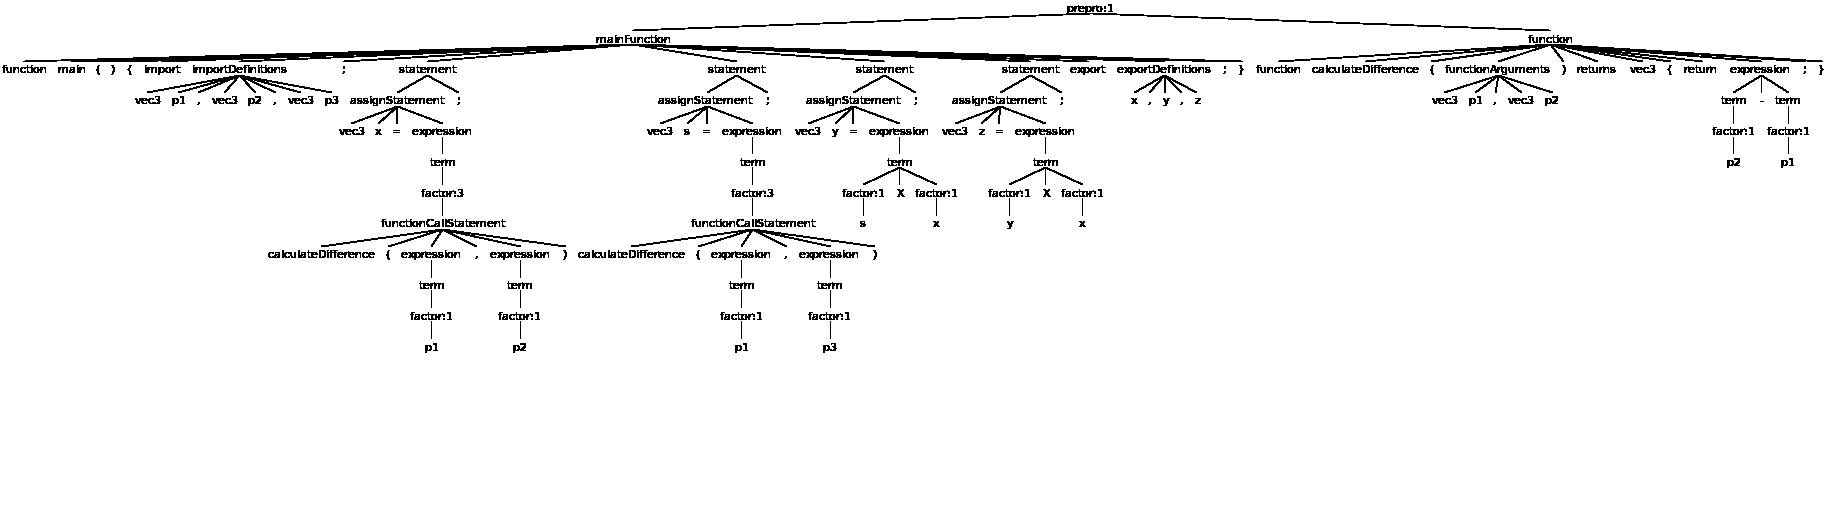
\includegraphics[width=\textwidth]{figures/parseTree}
	\caption{Beispielhafter \ac{AST}}
	\label{fig:AST_Example}
\end{figure}

\begin{lstlisting}[language=prepro, label={lst:AST_Example}, caption={PrePro-Code für den beispielhaften AST}, captionpos=b]
function main() {
    import vec3 p1;

    vec3 result = double(p1);
    result = result - p1;
    result = result - p1;

    export result;
}

function double(vec3 vec) returns vec3 {
    return add(vec, vec);
}

function add(vec3 a, vec3 b) returns vec3 {
    return a + b;
}
\end{lstlisting}
Ein \ac{AST}-Baum besteht nicht aus lauter gleichen Knoten, sondern aus vielen verschiedenen Klassen.
In PrePro gibt es eine Vielzahl an verschiedener Knoten-Typen, welche durch Java-Klassen repräsentiert werden.
Die Klassenhierarchie ist in \abb{fig:NodesHierachy} abgebildet.\\
Die dort aufgeführten Packages werden in den nachfolgenden Kapiteln im Detail erläutert.

\begin{figure}[H]
	\centering
	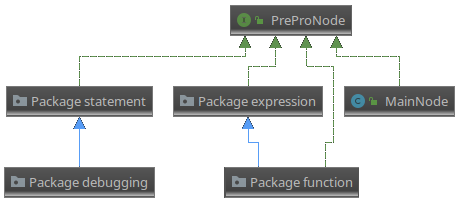
\includegraphics[width=\textwidth]{figures/uml_nodes}
	\caption{Die Knoten-Klassenhierarchie}
	\label{fig:NodesHierachy}
\end{figure}

\subsection{Wurzelknoten}
Die \texttt{MainNode} ist der Wurzelknoten des \ac{AST}.
Er beinhaltet als Kinder alle Funktionen, die in dem Programm definiert sind.
In Abbildung \abb{fig:AST_Example} sind die 3 Teilbäume ersichtlich, die den 3 Funktionen aus \code{lst:AST_Example} entsprechen.\\
Alle Knoten müssen das \texttt{PreProNode}-Interface implementieren.
Dieses ist ein leeres Interface, besitzt somit keine Funktionen und dient nur dazu, alle Knoten als Knoten zu markieren.

\subsection{Funktionen}
In PrePro gibt es Funktionen.
Direkt unter dem Wurzelknoten sind die Funktion-Knoten aufgehängt.
Sonst hängt nichts an dem Wurzelknoten.
Jede Funktion wird durch einen eigenen Knoten mitsamt Kindern dargestellt.
Zum Starten des Programms wird die Main-Funktion aus dem \ac{AST} herausgesucht und gestartet.
Eine Funktion hat Argumente, die ihr übergeben werden, diese müssen als Unterknoten in dem \ac{AST} gespeichert werden, damit sie bei der späteren Ausführung mit in die Funktion rein gegeben werden können.\\
Es wurde eine allgemeines \texttt{Function}-Interface definiert, welches die Funktionen \texttt{String getFunctionName()} und\\ \texttt{Variable execute(Arguments arguments, FunctionTable functionTable)} besitzt.\\
Das hat den Vorteil, dass das Interface unabhängig davon verwendet werden kann, ob die Funktion im Sourcecode definiert wurde oder von PrePro in Java-Code global zur Verfügung gestellt wurde.
Im ersteren Fall erzeugt der Parser eine \texttt{FunctionNode}, im zweiten Fall wird die Funktion in reinem Java spezifiziert.
Die \texttt{FuntionNode} führt die im Sourcecode angegebeben Statement-Nodes aus, die \texttt{CustomFunctionNode} ruft Java-Funktionen mittels Reflection auf.\\
Alle eben genannten Klassen sind im \texttt{nodes.function} Package abgelegt.

\subsection{Statements}
Eine Funktion besteht aus einer Reihe von Statements.
Eine Statement ist eine Anweisung, die ausgeführt wird und keine Rückgabe besitzt.
Dies grenzt sie von Expressions ab, die einen Wert zurückgeben.
Die Zeile \texttt{a = 1 + 2;} ist in ihrer Gesamtheit ein Statement, da es keine Rückgabe.\\
Als allgemeines Statement wurde die abstrakte Klasse \texttt{StatementNode} definiert.
Sie besitzt die Funktion\\ \texttt{void execute(SymbolTable symbolTable, FunctionTable functionTable)}
Alle Klassen, die von dieser Klasse erben, müssen die \texttt{execute}-Funktion implementieren.
Dazu zählt z.B. die \texttt{PrintStatementNode}, welche in der \texttt{execute}-Funktion einen Ausgabe auf dem Bildschirm erzeugen.

\subsection{Expression}
Die Teil \texttt{1 + 2} der Zeile \texttt{a = 1 + 2;} ist eine Expression.
Eine Expression ist ein (mathematischer) Ausdruck, der ausgeführt werden kann und einen Rückgabewert besitzt.
In einer Expression können neben mathematischen Operatoren, Konstanten, Variablen und Funktionsaufrufe beinhalten.
Die abstrakte Superklasse \texttt{ExpressionNode} definiert die Funktion\\
\texttt{Variable execute(SymbolTable symbolTable, FunctionTable functionTable)}.\\
Wichtig ist an dieser Stelle, dass die Funktion im Gegensatz zu der Funktion bei der \texttt{StatementNode} einen Wert vom allgemeinen Typ \texttt{Variable} zurück liefert.
Alle dafür nötigen Klassen sind in dem Package \texttt{nodes.expression} abgelegt.

\subsection{Debugging}
In PrePro ist zunächst eine rudimentäre Debugging-Möglichkeit eingebaut.
Es ist möglich an einer beliebigen Zeile im Code ein \texttt{break;} zu schrieben.
Bei der Ausführung stoppt der Interpreter in dieser Zeile und bietet eine kleine Kommandozeile um Variablen zu lesen und zu modifizieren.
Dieses Break-Statement ist ein Statement, erbt also von der \texttt{StatementNode}.
In der überschriebenen \texttt{execute}-Funktion wird auf die Eingabe und das Weiterspringen des Nutzers gewartet.

\section{Typsystem}
Das Typsystem von PrePro ist in \abb{fig:Typsystem} dargestellt.
Alle Variablen erben von er abstrakten Klasse \texttt{Variable}.
Es gibt die Untertypen \texttt{Vector}, \texttt{Marix}, \texttt{Scalar} und \texttt{Constant}.
Die Unterklassen \texttt{Vector} und \texttt{Matrix} haben wiederum Unterklassen für drei- und vierelementige Varianten.
Diese Unterklassen sind wichtig, da z.B. eine \texttt{Matrix3} mit einem \texttt{Vector3} multipliziert werden kann, allerdings nicht mit einem \texttt{Vector4}.\\
In der abstrakten Klasse \texttt{Variable} sind die Funktionen \texttt{add}, \texttt{sub}, \texttt{mul} und \texttt{div} definiert.
Werden die Funktionen auf der abstrakten Klasse aufgerufen, werfen sie eine Exception, dass die mathematische Operation nicht definiert sei.\\
Die Unterklassen haben nun die Möglichkeit, Operationen mit anderen Typen zu definieren.
Mittels Polymorphie und dynamic dispatching wird bei einer arithmetischen Operation die passende Funktion gesucht.
Falls keine passende Funktion wird die allgemeine - in der abstrakten Klasse definierte - Funktion verwendet, und daraufhin eine Exception geworfen, dass die mathematische Operation nicht definiert sei.

\begin{figure}[H]
	\centering
	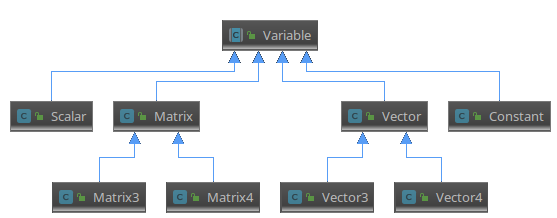
\includegraphics[width=\textwidth]{figures/typsystem}
	\caption{Typsystem von PrePro}
	\label{fig:Typsystem}
\end{figure}

\subsection{Darstellung der Typen in Java}
Alle Typen werden als \texttt{INDArray} von \texttt{ND4J} dargestellt.\\
Die Unterklassen besitzen einen Konstruktor, der ein \texttt{INDArray} übergeben bekommt.
In den Konstruktoren wird jeweils geprüft, ob die Dimensionen dem entsprechenden Typ entsprechen (z.B eine Matrix4 muss eine 4x4-Matrix übergeben bekommen).
Die einzige Ausnahme bildet der Typ ``Constant'', dieser bietet zusätzlich einen Konstruktur, dem ein \texttt{double} übergeben werden kann.
Intern wird aus dem \texttt{double} ein \texttt{INDArray} erzeugt.

\section{Implementierung der Operationen auf den Variablen-Typen}
In dem vorherigen Abschnitt wurden verschiedene Variablen-Typen herausgearbeitet.
Diese sind in \abb{fig:Typsystem} abgebildet.\\
Zwischen manchen der Typen sind Operationen, wie z.B. das Kreuzprodukt definiert.
Manche Typen können allerdings nicht sinnvoll kombiniert werden, z.B. eine Matrix3 und eine Matrix4.
Diese Operationen müssen in Java implementiert werden.
Ein erster Ansatz ist es, jedem Variablen-Typ die möglichen Operationen der Java-Klasse hinzuzufügen.
Dieser Ansatz wurde in dem \code{lst:Operationen_Matrix4} beispielsweise für die \texttt{Matrix4}-Klasse angewandt. Die Methoden sind jedoch lange nicht vollzählig.
\begin{lstlisting}[escapeinside={\%*}{*)},language=java, label={lst:Operationen_Matrix4}, caption={Implementierung der Operatoren in der Java-Klasse Matrix4}, captionpos=b]
%*
\begin{minted}[frame=single,framesep=10pt]{java}
public class Matrix4 {

	// same for sub, mul and div
	public Matrix4 add(Matrix4 right) {
		return new Matrix4(/* ... */);
	}

	// same for sub, mul and div
	public Matrix4 add(Constant right) {
		return new Matrix4(/* ... */);
	}

	// Cross-Product
	public Vector4 mul(Vector4 right) {
		return new Vector4(/* ... */);
	}
}
\end{minted}
\end{lstlisting}
Es ist zu erkennen, dass sehr viele Funktionen angelegt werden müssen.
Damit der Java-Compiler korrekt compilieren kann, müssen diese Funktionen in der Basisklasse \texttt{Variable} definiert werden und in den Unterklassen überschrieben werden.
Dies hat den Vorteil, dass in der Basis-Funktion in der Basis-Klasse \texttt{Variable} als normales Verhalten eine Fehlerausgabe erzeugt, in der gesagt wird, dass diese Operation auf diesen Typen nicht möglich ist.
In den Subklassen werden nun die Operatoren überschrieben und so das Standardverhalten der Fehlermeldung überschrieben.\\
Dieser Ansatz hätte zusätzlich den Vorteil, dass man Operatoren auch auf Klassen in der Mitte der Hierarchie - z.B. ein allgemeiner Vektor - anwenden kann. So kann die Vektoraddition an einer zentralen Stelle für \texttt{Vector3} und \texttt{Vector4} erfolgen.\\

\subsection{Dynamic Dispatching}
In der Theorie würde der aufgeführte Ansatz perfekt funktionieren.\\
Warum in der Theorie?
Dies allgemeine Problem wird in \code{lst:Dynamic_Dispatching} ersichtlich.

\begin{lstlisting}[escapeinside={\%*}{*)},language=java, label={lst:Dynamic_Dispatching}, caption={Java-Code zur Illustrierung von Dynamic Dispatching}, captionpos=b]
%*
\begin{minted}[frame=single,framesep=10pt]{java}
public class Main {

    public static void main(String[] args) {
        Dog dog1 = new Dog();
        test(dog1);
        Animal dog2 = new Dog();
        test(dog2);
    }

    private static void test(Animal a) {
        System.out.println("I'm an animal");
    }

    private static void test(Dog g) {
        System.out.println("I'm an dog");
    }
}

class Animal { }

class Dog extends Animal { }
\end{minted}
\end{lstlisting}
Das erwartete Verhalten wäre zwei Mal die Ausgabe ``I'm a dog''.\\
Die tatsächliche Ausgabe ist aber ``I'm a dog'' gefolgt von ``I'm a animal''.\\
Warum das?
Java entscheidet schon zur Kompilierzeit, welche Funktion aufgerufen wird.
Da zur Kompilierzeit noch nicht klar sein kann, welcher genaue Typ sich in der Variable \texttt{dog2} befindet, wird die die am besten passende Funktion für den deklarierten Typ der Variable verwendet. In diesem Fall ist die Variable \texttt{dog2} als \texttt{Animal} deklariert, deshalb wird die Funktion mit dem Parameter-Typ \texttt{Animal} ausgewählt.\\
Die Auswahl der Methode zur Laufzeit anhand des konkreten Typs statt zur Kompilierzeit nennt man \texttt{Dynamic Dispatching}.\\

\subsection{Groovy}
Eine Programmiersprache, die Dynamic Dispatching unterstützt ist Groovy.
Groovy wurde 2007 offiziell herausgegeben und ist syntax-kompatibel zu Java.
Der Code aus \code{lst:Dynamic_Dispatching} kann 1:1 in Groovy ausgeführt werden und erzeugt dort die erwartete Ausgabe von zwei mal ``I'm a dog''.
Groovy sucht sich die aufzurufende Funktion zur Laufzeit anhand des konkreten Typs raus.\\
Da Groovy syntax-kompatibel zu Java ist, wurde Groovy in das PrePro-Projekt aufgenommen.
Bestehende Klassen konnten übernommen werden.
Es wird allerdings darauf geachtet, dass der geschriebene Code Groovy (offensichtlich) und Java-kompatibel ist.
Dadurch wird die Lesbarkeit erhöht, da keine ständiger Wechsel zwischen Java und Groovy-Syntax notwendig ist.

\subsection{Bauen von Java und Groovy Projekten}
Da die \texttt{ND4j}-Bibliothek in Java geschrieben ist, wird versucht - sofern möglich - alles in Java zu schreiben.
Groovy wird nur in den Klassen verwendet, wo es benötigt wird.
Hierfür ist zu beachten, dass dies nicht nur die Klassen mit den Variable-Typen selber sind, sondern alle Klassen, die die Funktionen mittels Dynamic Dispatching aufrufen wollen.
Dadurch entsteht ein Projekt, welches Java und Groovy-Sourcecode beinhaltet.
Das PrePro-Projekt wird mittels Maven verwaltet und kompiliert.
Maven musste dafür das Plugin \texttt{org.codehaus.gmavenplus.gmavenplus-plugin} hinzugefügt werden, welches das Compilieren übernimmt.

\section{FunctionTable}
Ein PrePro-Programm besteht aus mehreren Funktionen.
Die Funktionen werden - auf den Namen indiziert - in einer FunctionTable gespeichert.
Aktuell ist diese als \texttt{HashMap<String, Function>} implementiert, weshalb Funktionen anhand ihrem Namen identifiziert werden. 
Damit ist aktuell kein Überladen von Funktionen möglich.
Falls ein Überladen ermöglicht werden soll, muss statt dem Namen ein Tupel aus Namen und Signatur der Funktion verwendet werden.
Auch muss bei dem Aufruf einer Funktion nicht nur nach dem Namen, sondern auch der Signatur geschaut werden.\\
Aufgrund dem Aufwand der Implementierung wurde dies in der ersten Version von PrePro nicht umgesetzt.
Die Sprache wurde jedoch mit dem Gedanken im Hinterkopf entwickelt, sodass die oben genannten Maßnahmen umgesetzt werden können und ein Überladen möglich wird.

\section{SymbolTable}
In einem PrePro-Programm können Variablen als Zwischenspeicher verwendet werden.
Die Symboltabelle ist bei dem PrePro-Interpreter ein Speicherplatz für diese Variablen.
Die Symboltabelle ist als \texttt{HashMap<String, Variable>} implementiert.
Aus ihr können die aktuellen Werte der Variablen gelesen und geschrieben werden.
Durch Auslesen des Typs, der in der Symboltabelle gespeichert ist, kann der Typ der Variable ermittelt werden.\\
Jede Funktion erstellt zu Beginn der Ausführung der Funktion eine Symboltabelle und fügt die übergebenen Parameter hinzu.
Anschließend wird auf der Symboltabelle die Funktion abgearbeitet.
Ist die Funktion fertig abgearbeitet wird der Rückgabewert aus der Symboltabelle berechnet, die Symboltabelle wird anschließend verworfen.
Hat eine Funktion keinen Rückgabewert, entfällt der Berechnungsschritt für die Rückgae dementsprechend.
\\
Es ist möglich eine bereits gefüllte Symboltabelle bei dem Start eines PrePro-Programms mitzugeben.
Diese steht dann in der Main-Funktion direkt zur Verfügung.
So kann z.B. eine Symboltabelle mit Konstanten einmal aufgebaut und dann von mehreren PrePro-Programmen wiederverwendet werden.

\section{Grundrechenarten}
Bei der Darstellung der Zahlen im Speicher wird für jede Zahl ein Double verwendet.
Das erhöht die Genauigkeit gegenüber einem float und erspart Konvertierungen zwischen Ganz- und Fließzahlen.
Grundrechenarten sind die Addition, Subtraktion, Multiplikation und Division von Matrizen.
Diese Operationen sind elementweise und werden direkt von ND4J zur Verfügung gestellt und können aufgerufen werden.

\section{Kreuzprodukt}
Anders als die vier Grundarten aus dem vorherigen Abschnitt wird das Kreuzprodukt von ND4J nicht als Operation angeboten.
Das Kreuzprodukt wird in der Praxis allerdings zu Beispiel für das Aufspannen von Vektoren im dreidimensionalen Raum benötigt.
Daher wird an dieser Stelle das Kreuzprodukt zweier Vektoren selber implementiert.
Falls ND4J in Zukunft den Operator Kreuzprodukt bereit stellt, kann in zukünftigen Varianten auf ihre Implementierung zugegriffen werden, da diese wahrscheinlich effizienter sein wird.
Die eigene Implementierung des Kreuzprodukts kann auf folgende Arten geschehen:
\begin{enumerate}
	\item Implementierung in Plain Java mittels einer for-Schleife.
	\item Implementierung in Plain Java mittels Subarrays
\end{enumerate}

\subsection{Implementierung Kreuzprodukt mittels For-Schleife}
Bei der Implementierung mittels der For-Schleife werden die eigentlichen Berechnungen in Java durchgeführt.
Als erstes wird ein Double-Array als Zwischenspeicher für das Ergebnis angelegt.
Es besitzt (Anzahl der Zeitelemente in den Eingabe-Vektoren) * drei Elemente.
Die Anzahl der Elemente entspricht so der Anzahl der Elemente der Ergebnismatrix, die Daten können in dem Double-Array effizient gespeichert werden.
Das Array wird im Anschluss in eine Matrix konvertiert.
Für die Berechnung der Elemente wird mittels einer For-Schleife über alle Zeilen der Matrix iteriert.
In jeder Zeile werden die 3 Werte des entstehenden Ergebnisvektors berechnet und in das Double-Array gespeichert.
Abschließend wir das Double-Array in eine Matrix mit den Dimensionen [<Anzahl Zeitelemente> x drei] konvertiert und durch eine Vector3-Wrapper-Klasse als Vector mit 3 Werten gekennzeichnet.
Der Algorithmus ist in \code{lst:Kreuzprodukt_For} dargestellt.

\begin{lstlisting}[escapeinside={\%*}{*)},language=java, label={lst:Kreuzprodukt_For}, caption={Implementierung Kreuzprodukt mittels for-Schleife}, captionpos=b]
%*
\begin{minted}[frame=single,framesep=10pt,breaklines]{java}
private Vector3 crossProduct(Vector3 left, Vector3 right) {
    INDArray a = left.getNdArray();
    INDArray b = right.getNdArray();

    int size = a.shape()[0];
    double[] result = new double[size * 3];

    for (int i = 0; i < size; i++) {
        result[i * 3 + 0] = a.getDouble(i, 1) * b.getDouble(i, 2) - a.getDouble(i, 2) * b.getDouble(i, 1);
        result[i * 3 + 1] = a.getDouble(i, 2) * b.getDouble(i, 0) - a.getDouble(i, 0) * b.getDouble(i, 2);
        result[i * 3 + 2] = a.getDouble(i, 0) * b.getDouble(i, 1) - a.getDouble(i, 1) * b.getDouble(i, 0);
    }
    return new Vector3(Nd4j.create(result, new int[]{size, 3}));
}
\end{minted}
\end{lstlisting}

\subsection{Implementierung Kreuzprodukt mittels Subarrays}
\begin{lstlisting}[escapeinside={\%*}{*)},language=java, label={lst:Kreuzprodukt_Subarray}, caption={Implementierung Kreuzprodukt mittels for-Schleife}, captionpos=b]
%*
\begin{minted}[frame=single,framesep=10pt,breaklines]{java}
private Vector3 crossProductSubArray(Vector3 left, Vector3 right) {
    INDArray a = left.getNdArray();
    INDArray b = right.getNdArray();

    INDArray a1 = a.getColumn(0);
    INDArray a2 = a.getColumn(1);
    INDArray a3 = a.getColumn(2);

    INDArray b1 = b.getColumn(0);
    INDArray b2 = b.getColumn(1);
    INDArray b3 = b.getColumn(2);

    INDArray c1 = (a2.mul(b3)).sub(a3.mul(b2));
    INDArray c2 = (a3.mul(b1)).sub(a1.mul(b3));
    INDArray c3 = (a1.mul(b2)).sub(a2.mul(b1));

    int size = a.shape()[0];
    INDArray result = Nd4j.create(size, 3);
    result.putColumn(0, c1);
    result.putColumn(1, c2);
    result.putColumn(2, c3);

    return new Vector3(result);
}
\end{minted}
\end{lstlisting}

\section{Vergleich der Implementierungen für Kreuzprodukt}
Beide Impelemtierungsmöglichkeiten haben Vor- und Nachteile.
Diese sind in \tab{tab:Vorteile_Kreuzprodukt_Implementierungen} aufgeführt.
\begin{table}[H]
	\centering
	\begin{tabular}{ | p{4cm} | p{5.5cm} | p{5.5cm} | }
		\hline \rowcolor{gray!15}
		\textbf{Implementierungs-möglichkeit} & \textbf{Vorteile} & \textbf{Nachteile} \\ \hhline{|=|=|=|}
		Mittels For-Schleife & Leichter verständlich. & Wird direkt in Java ausgeführt. \newline Mögliche Optimierungen von ND4J können nicht verwendet werden. Berechnungen finden nur auf der \ac{CPU} statt! \\ \hline
		Mittels Subarray & Durch die Verwendung von ND4J können die Optimierungen verwendet werden. Wenn ND4J so konfiguriert ist, dass es auf der \ac{GPU} läuft, kann die eigentliche Berechnung weiterhin auf der \ac{GPU} erfolgen. & Schwerer verständlich. \\ \hline
	\end{tabular}
	\caption{Vor- und Nachteile einer Implementierung mittels Compiler oder Interpreter}
	\label{tab:Vorteile_Kreuzprodukt_Implementierungen}
\end{table}

\noindent Für große Zeitreihen müsste sich die Implementierung mittels dem Subarray als effizienter erweisen, besonders wenn die Berechnungen auf der \ac{GPU} durchgeführt werden.
Als Nachweis und für das Effizienzverhalten bei kleinen Zeitreihen wurde ein Benchmark durchgeführt.
Die Ergebnisse sind in \tab{tab:Benchmark_Kreuzprodukt_Implementierung} festgehalten.

\begin{table}[H]
	\centering
	\begin{tabular}{ | p{5cm} | p{3.5cm} | p{3.5cm} | }
		\hline \rowcolor{gray!15}
		\textbf{Anzahl Datensätze} & \textbf{For-Schleife} & \textbf{Subarray} \\ \hhline{|=|=|=|}
		100 & 6 (342) & 4 (13) \\ \hline
		1.000 & 20 (489) & 7 (22) \\ \hline
		10.000 & 53 (527) & 5 (21) \\ \hline
		100.000 & 333 (1159) & 5 (15) \\ \hline
		1.000.000 & 3205 (4129) & 47 (64) \\ \hline
		10.000.000 & 32358 (33594) & 442 (453) \\ \hline

	\end{tabular}
	\caption[Benchmark-Ergebnisse der verschiedenen Implementierungsmöglichkeiten für das Kreuzprodukt]
	{Benchmark-Ergebnisse der verschiedenen Implementierungsmöglichkeiten für das Kreuzprodukt. Die Messung ist nach 5 Durchläufen in Millisekunden gemessen, die Zahl in Klammern gibt die Zeit des ersten Durchlaufs an.}
	\label{tab:Benchmark_Kreuzprodukt_Implementierung}
\end{table}

3 Varianten

Benchmarks!
Klassifizierung \ac{CPU} oder \ac{GPU}-Workload.

Möglicherweise lohnt sich die eher \ac{GPU}-betonte Variante erst ab gewisser Größe.
=> Dann mit konstantem Aufwand entscheiden, welches Verfahren.
Vom Nutzer (während Laufzeit) auswählbar?
%%%%%%%%%%%%%%%%%%%%%%%%%%%%%%%%%%%%%%%%%%%%%%%%%%%%%%%%%%%%%%%%%%%%%%%%%%%%%%%
\endinput
%%%%%%%%%%%%%%%%%%%%%%%%%%%%%%%%%%%%%%%%%%%%%%%%%%%%%%%%%%%%%%%%%%%%%%%%%%%%%%%
